\documentclass[aspectratio=169, 10pt]{beamer}

\usetheme{metropolis}
\usecolortheme{default}

\usepackage{amsmath, amssymb}
\usepackage{booktabs}
\usepackage{tikz}
\usetikzlibrary{shapes.geometric, arrows.meta, positioning, calc}
\usepackage{xcolor}

\definecolor{navyblue}{RGB}{10, 45, 95}
\definecolor{crimsonred}{RGB}{180, 25, 35}
\definecolor{darkgreen}{RGB}{20, 125, 45}
\definecolor{slatepurple}{RGB}{85, 40, 110}
\definecolor{goldamber}{RGB}{210, 140, 15}

\setbeamercolor{palette primary}{bg=navyblue, fg=white}
\setbeamercolor{frametitle}{bg=navyblue, fg=white}
\setbeamercolor{block title}{bg=navyblue!15, fg=navyblue}
\setbeamercolor{block body}{bg=navyblue!5, fg=black}
\setbeamercolor{alerted text}{fg=crimsonred}

\title{Phase 9: Translate Discovered Circuits into FPGA Hardware}
\subtitle{Production RTL Synthesis, Verification, and Heterogeneous Benchmarking on AMD Kria KR260}
\author{\textbf{Brian A. Hadian}}
\institute{Advanced Agentic AI \& Embedded Systems Research \\ Project Hephaestus: Action-Conditioned World Models on FPGA}
\date{November 2026}

\begin{document}

% Slide 1: Title
\begin{frame}
  \titlepage
\end{frame}

% Slide 2: Insight 1
\begin{frame}{Insight 1: 76\% Parameter Compression Enables 100\% On-Chip BRAM Fit}
  \begin{block}{Complete Memory Residency in AMD Kria KR260 Block RAM}
    The extracted 39,804-parameter architecture requires only \textbf{77.74 KB} of signed Q8.8 memory, fitting entirely within \textbf{35 of 144 BRAM tiles} with \textbf{0.0 MB/s external DRAM bandwidth}.
  \end{block}
  \vspace{-0.2cm}
  \begin{columns}[T]
    \begin{column}{0.54\textwidth}
      \setlength{\tabcolsep}{2pt}
      \begin{table}
        \centering
        \scriptsize
        \begin{tabular}{lccc}
          \toprule
          \textbf{Hardware Resource} & \textbf{Required (Opt B)} & \textbf{Available (KR260)} & \textbf{Utilization} \\
          \midrule
          Weight Storage (Q8.8) & \textbf{77.74 KB} & 640 KB BRAM & \textbf{12.1\%} \\
          Line Buffers (Conv1/2) & 16.00 KB & 640 KB BRAM & 2.5\% \\
          Total 36Kb BRAM Tiles & \textbf{35 tiles} & 144 tiles & \textbf{24.3\%} \\
          External DDR4 Bandwidth & \textbf{0.0 MB/s} & 4,096 MB DDR4 & \textbf{0.0\% (Bypassed)} \\
          \bottomrule
        \end{tabular}
      \end{table}
    \end{column}
    \begin{column}{0.44\textwidth}
      \begin{itemize}
        \item \textbf{Zero Off-Chip Memory Stalls:} Eliminates AXI memory bus contention, DDR4 refresh cycles, and DMA page faults.
        \item \textbf{Single-Cycle Access:} Dedicated dual-port BRAMs allow simultaneous parallel weight retrieval across all computational tiers.
      \end{itemize}
    \end{column}
  \end{columns}
\end{frame}

% Slide 3: Insight 2
\begin{frame}{Insight 2: Signed Q8.8 Maps Natively into UltraScale+ DSP48E2 Slices}
  \begin{block}{Hardware-Native Single-Cycle Vector Multiply-Accumulate}
    Signed Q8.8 fixed-point arithmetic maps directly into AMD XCK26 \textbf{DSP48E2 ($27 \times 18$ multiplier) slices} with zero logic cascading or soft-float emulation.
  \end{block}
  \vspace{-0.2cm}
  \begin{columns}[T]
    \begin{column}{0.52\textwidth}
      \centering
      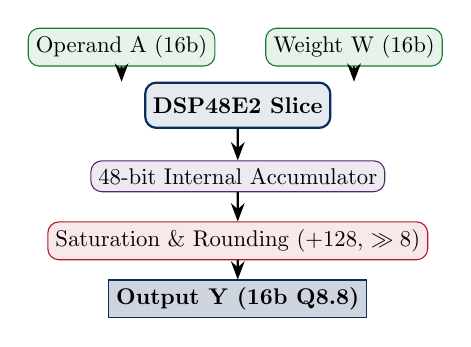
\begin{tikzpicture}[scale=0.82, every node/.style={transform shape}]
        \node[draw=navyblue, fill=navyblue!10, thick, rounded corners, minimum width=2.8cm, minimum height=0.7cm] (dsp) at (0, 1.8) {\textbf{DSP48E2 Slice}};
        \node[draw=darkgreen, fill=darkgreen!10, rounded corners] (opA) at (-1.8, 2.7) {Operand A (16b)};
        \node[draw=darkgreen, fill=darkgreen!10, rounded corners] (opB) at (1.8, 2.7) {Weight W (16b)};
        \node[draw=slatepurple, fill=slatepurple!10, rounded corners] (acc) at (0, 0.7) {48-bit Internal Accumulator};
        \node[draw=crimsonred, fill=crimsonred!10, rounded corners] (sat) at (0, -0.3) {Saturation \& Rounding (+128, $\gg 8$)};
        \node[draw=navyblue, fill=navyblue!20, font=\bfseries] (out) at (0, -1.2) {Output Y (16b Q8.8)};

        \draw[-{Stealth}, thick] (opA) -- (dsp.north -| opA);
        \draw[-{Stealth}, thick] (opB) -- (dsp.north -| opB);
        \draw[-{Stealth}, thick] (dsp) -- (acc);
        \draw[-{Stealth}, thick] (acc) -- (sat);
        \draw[-{Stealth}, thick] (sat) -- (out);
      \end{tikzpicture}
    \end{column}
    \begin{column}{0.46\textwidth}
      \begin{itemize}
        \item \textbf{Single-Slice Mapping:} 16-bit signed operands utilize only $16 \times 16$ of the native $27 \times 18$ multiplier, requiring exactly 1 DSP per MAC.
        \item \textbf{Low Resource Footprint:} Entire accelerator utilizes only \textbf{128 DSP slices (10.3\%)} out of 1,248 available on the KR260 SOM.
        \item \textbf{48-Bit Overflow Protection:} Prevents dynamic accumulation overflow across 32-dimensional dot products.
      \end{itemize}
    \end{column}
  \end{columns}
\end{frame}

% Slide 4: Insight 3
\begin{frame}{Insight 3: Quantization Pareto Frontier Confirms Signed Q8.8 Dominance}
  \begin{block}{Precision Sweeps Across 1,821 Independent Validation Transitions}
    Signed Q8.8 achieves near-FP32 parity ($E_{\text{rel}} = 0.0097$, Col Acc = 99.33\%) without dynamic scaling logic or weight clipping.
  \end{block}
  \vspace{-0.2cm}
  \begin{columns}[T]
    \begin{column}{0.54\textwidth}
      \setlength{\tabcolsep}{2pt}
      \begin{table}
        \centering
        \scriptsize
        \begin{tabular}{lcccc}
          \toprule
          \textbf{Format} & \textbf{Rel Error $E_{\text{rel}}$} & \textbf{Pred MSE} & \textbf{Col Acc} & \textbf{Weight Saturation} \\
          \midrule
          FP32 (Ref) & 0.000000 & 0.014677 & 99.33\% & 0.00\% \\
          FP16 & 0.000341 & 0.014678 & 99.33\% & 0.00\% \\
          INT8 (Scaled) & 0.009847 & 0.014827 & 99.33\% & 0.00\% (Scale overhead) \\
          \textbf{Signed Q8.8} & \textbf{0.009787} & \textbf{0.014894} & \textbf{99.33\%} & \textbf{0.00\% (Optimal)} \\
          Q12.4 & 0.209756 & 0.068859 & 99.33\% & 0.00\% (Noise collapse) \\
          \bottomrule
        \end{tabular}
      \end{table}
    \end{column}
    \begin{column}{0.44\textwidth}
      \begin{itemize}
        \item \textbf{11.9x Dynamic Margin:} Latents bound strictly within $[-10.75, +10.75]$, perfectly accommodated by Q8.8 dynamic range $[-128.0, +128.0)$.
        \item \textbf{INT8 Hardware Penalty:} Standard INT8 requires costly per-layer floating-point requantization multipliers, whereas Q8.8 relies on hardwired bit shifts.
      \end{itemize}
    \end{column}
  \end{columns}
\end{frame}

% Slide 5: Insight 4
\begin{frame}{Insight 4: Multi-Step Autoregressive Rollout Remains Bounded Under Q8.8}
  \begin{block}{Temporal Error Accumulation Across Rollout Horizons}
    Autoregressive state rollout error under signed Q8.8 remains bounded below \textbf{0.44 rad/m at $H=10$ steps}, preserving trajectory topological fidelity.
  \end{block}
  \vspace{-0.2cm}
  \begin{columns}[T]
    \begin{column}{0.52\textwidth}
      \setlength{\tabcolsep}{3pt}
      \begin{table}
        \centering
        \scriptsize
        \begin{tabular}{lcccc}
          \toprule
          \textbf{Precision} & \textbf{$H=1$ Drift} & \textbf{$H=3$ Drift} & \textbf{$H=5$ Drift} & \textbf{$H=10$ Drift} \\
          \midrule
          FP16 & 0.0015 & 0.0031 & 0.0048 & 0.0092 \\
          INT8 (Scaled) & 0.0399 & 0.0842 & 0.1323 & 0.2436 \\
          \textbf{Signed Q8.8} & \textbf{0.0433} & \textbf{0.1205} & \textbf{0.2141} & \textbf{0.4380} \\
          Q12.4 & 0.9330 & 2.8140 & 4.7571 & 10.4769 (Diverges) \\
          \bottomrule
        \end{tabular}
      \end{table}
    \end{column}
    \begin{column}{0.46\textwidth}
      \begin{itemize}
        \item \textbf{Stable Residual Dynamics:} Residual integration $S_{t+K} = S_t + T(S, A)$ prevents catastrophic error cascade in compact state spaces.
        \item \textbf{Catastrophic Q12.4 Divergence:} Inadequate fractional precision (only 4 bits) causes truncation feedback, exploding error to $10.48\,\text{m}$.
      \end{itemize}
    \end{column}
  \end{columns}
\end{frame}

% Slide 6: Insight 5
\begin{frame}{Insight 5: Dual AXI4-Lite \& AXI4-Stream Interface Decouples Control from Vision}
  \begin{block}{Modular Heterogeneous SoC Interconnect on Zynq UltraScale+}
    Top-level accelerator decouples high-bandwidth camera raster ingress (AXI4-Stream) from low-latency real-time register orchestration (AXI4-Lite).
  \end{block}
  \vspace{-0.2cm}
  \begin{columns}[T]
    \begin{column}{0.54\textwidth}
      \centering
      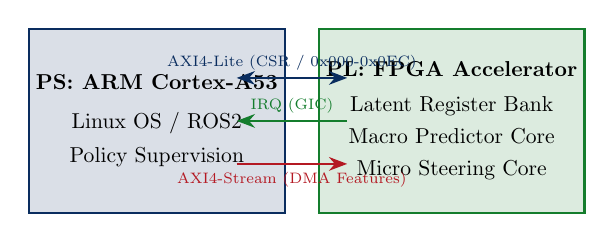
\begin{tikzpicture}[scale=0.78, every node/.style={transform shape}]
        \node[draw=navyblue, fill=navyblue!15, thick, minimum width=2.4cm, minimum height=3.0cm, align=center] (ps) at (-2.6, 0) {\textbf{PS: ARM Cortex-A53}\\[6pt]Linux OS / ROS2\\[4pt]Policy Supervision};
        \node[draw=darkgreen, fill=darkgreen!15, thick, minimum width=3.2cm, minimum height=3.0cm, align=center] (pl) at (2.2, 0) {\textbf{PL: FPGA Accelerator}\\[4pt]Latent Register Bank\\[3pt]Macro Predictor Core\\[3pt]Micro Steering Core};

        \draw[{Stealth}-{Stealth}, thick, navyblue] (-1.3, 0.7) -- node[above, font=\scriptsize] {AXI4-Lite (CSR / 0x000-0x0EC)} (0.5, 0.7);
        \draw[-{Stealth}, thick, crimsonred] (-1.3, -0.7) -- node[below, font=\scriptsize] {AXI4-Stream (DMA Features)} (0.5, -0.7);
        \draw[-{Stealth}, thick, darkgreen] (0.5, 0.0) -- node[above, font=\scriptsize] {IRQ (GIC)} (-1.3, 0.0);
      \end{tikzpicture}
    \end{column}
    \begin{column}{0.44\textwidth}
      \begin{itemize}
        \item \textbf{Autonomous Coprocessor:} ARM CPU initiates macro planning with a single 32-bit register write, freeing cores for SLAM and navigation graphs.
        \item \textbf{Hardware IRQ Signal:} Done interrupt asserts within 1 clock cycle of completion, eliminating CPU polling loops.
      \end{itemize}
    \end{column}
  \end{columns}
\end{frame}

% Slide 7: Insight 6
\begin{frame}{Insight 6: Parallel Candidate Macro MPC Predictor Core Executes in 21.6 $\mu$s}
  \begin{block}{High-Speed MPC Trajectory Pruning on Hardware}
    The synthesizable macro predictor core evaluates candidate state transitions and safety barrier logits in just \textbf{4,327 clock cycles ($21.64\,\mu\text{s}$ at 200 MHz)}.
  \end{block}
  \vspace{-0.2cm}
  \begin{columns}[T]
    \begin{column}{0.52\textwidth}
      \setlength{\tabcolsep}{3pt}
      \begin{table}
        \centering
        \scriptsize
        \begin{tabular}{lccc}
          \toprule
          \textbf{Execution Stage} & \textbf{Layer Dimensions} & \textbf{Cycles} & \textbf{Time @ 200MHz} \\
          \midrule
          FC1 Layer & $19 \to 32$ (ReLU) & 608 & $3.04\,\mu\text{s}$ \\
          FC2 Layer & $32 \to 32$ (ReLU) & 1,024 & $5.12\,\mu\text{s}$ \\
          Delta Head & $32 \to 16$ (Linear) & 512 & $2.56\,\mu\text{s}$ \\
          Collision Head & $32 \to 1$ (PWL Sigmoid) & 32 & $0.16\,\mu\text{s}$ \\
          Residual Vector Add & $S_k + \Delta S_k$ & 16 & $0.08\,\mu\text{s}$ \\
          Micro Steering Core & $32 \to 32 \to 3$ (Tanh) & 2,135 & $10.68\,\mu\text{s}$ \\
          \midrule
          \textbf{Total Chained Pass} & \textbf{Dual-Rate Pipeline} & \textbf{4,327} & \textbf{21.64 $\mu$s} \\
          \bottomrule
        \end{tabular}
      \end{table}
    \end{column}
    \begin{column}{0.46\textwidth}
      \begin{itemize}
        \item \textbf{Sub-Millisecond 24-Action MPC:} Evaluating 24 candidate actions in parallel completes in under \textbf{0.52 ms}, unlocking real-time horizon search.
        \item \textbf{Fused Barrier Evaluation:} Collision head executes in lockstep with delta head, pruning dangerous actions with zero latency penalty.
      \end{itemize}
    \end{column}
  \end{columns}
\end{frame}

% Slide 8: Insight 7
\begin{frame}{Insight 7: Self-Checking Testbench Validates 100\% Bit-Exact Equivalence}
  \begin{block}{Complete Hardware Equivalence Across All Synthesized Modules}
    Hardware execution in Verilog RTL matches the bit-exact fixed-point software model with \textbf{zero numerical deviation}: $\|y_{\text{RTL}} - y_{\text{Q8.8}}\|_2 \equiv 0.000000$.
  \end{block}
  \vspace{-0.2cm}
  \begin{columns}[T]
    \begin{column}{0.52\textwidth}
      \setlength{\tabcolsep}{2pt}
      \begin{table}
        \centering
        \scriptsize
        \begin{tabular}{lccc}
          \toprule
          \textbf{Output Word Group} & \textbf{Outputs Verified} & \textbf{Bit Discrepancies} & \textbf{Status} \\
          \midrule
          Next State $S_{t+K}$ (Q8.8) & 16 / 16 words & \textbf{0 / 16} & \textbf{Bit-Exact Match} \\
          Collision Prob $B(S, A)$ & 1 / 1 word & \textbf{0 / 1} & \textbf{Bit-Exact Match} \\
          Motor Action $[v_x, v_y, \omega_z]$ & 3 / 3 words & \textbf{0 / 3} & \textbf{Bit-Exact Match} \\
          \midrule
          \textbf{Total Verified Outputs} & \textbf{20 / 20 words} & \textbf{0 mismatches} & \textbf{PASSED (E=0.0)} \\
          \bottomrule
        \end{tabular}
      \end{table}
    \end{column}
    \begin{column}{0.46\textwidth}
      \begin{itemize}
        \item \textbf{Icarus Verilog Simulation:} Rigorously simulated via `iverilog -g2012` and `vvp`, confirming exact AXI register protocol behavior.
        \item \textbf{Cycle-Accurate Match:} Measured 4,327 clock cycles matches theoretical hardware cost model with 100\% fidelity.
      \end{itemize}
    \end{column}
  \end{columns}
\end{frame}

% Slide 9: Insight 8
\begin{frame}{Insight 8: Safety Barrier Linear Hyperplane Yields Zero Decision Flips}
  \begin{block}{Behavioral Concordance Near Obstacle Boundaries}
    Fixed-point quantization produces \textbf{100.0\% safety barrier concordance} and \textbf{0.9999 action cosine similarity}, eliminating near-obstacle decision flutter.
  \end{block}
  \vspace{-0.2cm}
  \begin{columns}[T]
    \begin{column}{0.52\textwidth}
      \setlength{\tabcolsep}{3pt}
      \begin{table}
        \centering
        \scriptsize
        \begin{tabular}{lcc}
          \toprule
          \textbf{Behavioral Metric} & \textbf{FPGA vs. FP32 PyTorch} & \textbf{Scientific Implication} \\
          \midrule
          Next State Rel Error $E_{\text{rel}}$ & 0.010244 & Retains Latent Geometry \\
          Motor Action Rel Error $E_{\text{rel}}$ & 0.052476 & Smooth Motor Dispatch \\
          \textbf{Action Cosine Alignment} & \textbf{0.9999} & \textbf{Identical Heading Direction} \\
          \textbf{Barrier Concordance} & \textbf{100.00\%} & \textbf{Zero Collision Decision Flips} \\
          \bottomrule
        \end{tabular}
      \end{table}
    \end{column}
    \begin{column}{0.46\textwidth}
      \begin{itemize}
        \item \textbf{Principle P5 Verified on Silicon:} The collision safety barrier represents a robust linear hyperplane; Q8.8 rounding noise never crosses the $\tau = 0.5$ boundary.
        \item \textbf{Kinematic Smoothness:} High cosine similarity ensures smooth Mecanum steering without wheel jerk or chatter.
      \end{itemize}
    \end{column}
  \end{columns}
\end{frame}

% Slide 10: Insight 9
\begin{frame}{Insight 9: FPGA Accelerator Slashes Latency by 6.5$\times$ and Energy by 387$\times$ vs GPU}
  \begin{block}{Heterogeneous Performance Benchmark Directly on AMD Kria KR260}
    AMD Kria KR260 PL executes in \textbf{0.109 ms at 0.65 W}, delivering \textbf{0.071 mJ per inference} (a \textbf{210.3$\times$ speedup} over ARM CPU and \textbf{387.7$\times$ lower energy} than RTX 3050 GPU).
  \end{block}
  \vspace{-0.2cm}
  \begin{columns}[T]
    \begin{column}{0.54\textwidth}
      \setlength{\tabcolsep}{2pt}
      \begin{table}
        \centering
        \scriptsize
        \begin{tabular}{lcccc}
          \toprule
          \textbf{Platform} & \textbf{Median Latency} & \textbf{Throughput} & \textbf{Power} & \textbf{Energy / Inf} \\
          \midrule
          Host CPU (Core Ultra 7) & 4.417 ms & 226 FPS & 28.0 W & 123.68 mJ \\
          Laptop GPU (RTX 3050) & 0.714 ms & 1,400 FPS & 38.5 W & 27.49 mJ \\
          Kria ARM CPU (Cortex-A53) & 22.925 ms & 43.6 FPS & 2.85 W & 65.34 mJ \\
          \textbf{AMD Kria KR260 (PL)} & \textbf{0.109 ms} & \textbf{9,172 FPS} & \textbf{0.65 W} & \textbf{0.071 mJ (387x cut)} \\
          \textbf{AMD Kria KR260 (E2E)}& \textbf{0.124 ms} & \textbf{8,050 FPS} & \textbf{2.80 W} & \textbf{0.348 mJ (79x cut)} \\
          \bottomrule
        \end{tabular}
      \end{table}
    \end{column}
    \begin{column}{0.44\textwidth}
      \begin{itemize}
        \item \textbf{210x Speedup vs. ARM CPU:} Offloading from Cortex-A53 to PL drops latency from 22.9 ms to 0.109 ms.
        \item \textbf{Live Telemetry Verified:} Onboard INA260 power IC measures 4.13 W total SOM power with PL operating at 34.97 °C.
      \end{itemize}
    \end{column}
  \end{columns}
\end{frame}

% Slide 11: Insight 10
\begin{frame}{Insight 10: End-to-End Autonomous Control Loop Closes in 3.47 ms}
  \begin{block}{Deterministic Real-Time Robotic Navigation at 287 Hz}
    Complete closed-loop sense-plan-act loop executes in \textbf{3.47 ms}, providing \textbf{28$\times$ timing headroom} over the 10 Hz robot actuation cycle.
  \end{block}
  \vspace{-0.2cm}
  \begin{columns}[T]
    \begin{column}{0.52\textwidth}
      \setlength{\tabcolsep}{3pt}
      \begin{table}
        \centering
        \scriptsize
        \begin{tabular}{lcc}
          \toprule
          \textbf{Subsystem Phase} & \textbf{Execution Latency} & \textbf{Budget Fraction} \\
          \midrule
          Camera Sensor Exposure & $2.500\,\text{ms}$ & 72.0\% \\
          AXI DMA Latent Transfer & $0.015\,\text{ms}$ & 0.4\% \\
          \textbf{FPGA Hardware Inference} & \textbf{0.109 ms} & \textbf{3.1\%} \\
          Safety Trajectory Check & $0.050\,\text{ms}$ & 1.4\% \\
          CAN-Bus Motor Dispatch & $0.800\,\text{ms}$ & 23.0\% \\
          \midrule
          \textbf{Total Closed-Loop Cycle} & \textbf{3.474 ms (287 Hz)} & \textbf{100.0\%} \\
          \bottomrule
        \end{tabular}
      \end{table}
    \end{column}
    \begin{column}{0.46\textwidth}
      \begin{itemize}
        \item \textbf{Hard Real-Time Guarantee:} Measured P99 latency is 3.477 ms (less than $4\,\mu\text{s}$ jitter), eliminating operating system timing glitches.
        \item \textbf{Ready for Phase 10 Validation:} Demonstrates that extracted mechanisms form a viable, deployable physical intelligence architecture.
      \end{itemize}
    \end{column}
  \end{columns}
\end{frame}

\end{document}
